\documentclass[tikz,border=3pt]{standalone}
\usepackage[utf8]{inputenc}
\usepackage[T1]{fontenc}
\usepackage{lmodern}
\renewcommand{\familydefault}{\sfdefault}
\usepackage{sansmath}\sansmath
\usepackage{chemfig}
\usepackage{pgfplots}\pgfplotsset{compat=1.18,/pgf/number format/use comma,/pgf/number format/1000 sep={.}}
\usetikzlibrary{arrows.meta,calc,positioning,decorations.pathmorphing,patterns}
% paleta del sitio
\definecolor{nar}{HTML}{E8680C}\definecolor{narc}{HTML}{FFB35C}\definecolor{hielo}{HTML}{FFF3E8}
\definecolor{tinta}{HTML}{1D1D1F}\definecolor{gris}{HTML}{6E6E73}\definecolor{lila}{HTML}{7C5CF0}
\definecolor{azul}{HTML}{2F6FD6}\definecolor{menta}{HTML}{17A673}\definecolor{coral}{HTML}{E8342A}
\begin{document}
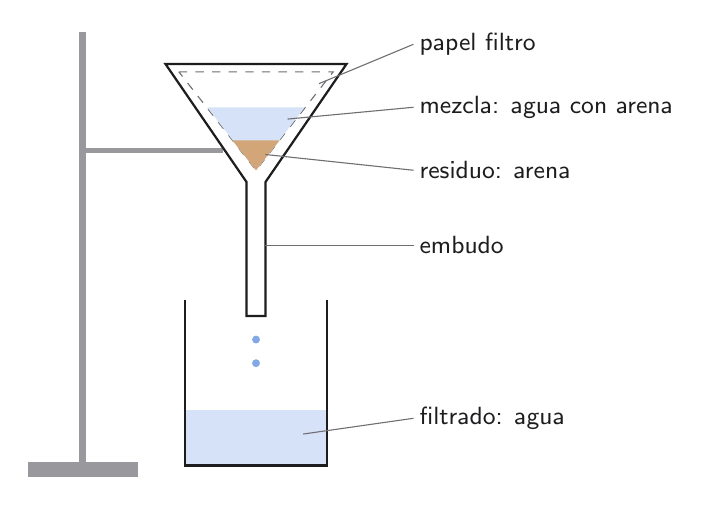
\begin{tikzpicture}[font=\small]

\fill[gris!70] (-2.9,-0.15) rectangle (-1.5,0.05);
\draw[gris!70,line width=2.5pt] (-2.2,0.05) -- (-2.2,5.5);

\draw[gris!70,line width=1.6pt] (-2.2,4.0) -- (-0.42,4.0);
\fill[azul!20] (-0.9,0) rectangle (0.9,0.7);
\draw[tinta,thick] (-0.9,2.1) -- (-0.9,0) -- (0.9,0) -- (0.9,2.1);
\draw[tinta,thick,fill=white] (-1.15,5.1) -- (1.15,5.1) -- (0.12,3.6) -- (0.12,1.9) -- (-0.12,1.9) -- (-0.12,3.6) -- cycle;
\draw[gris,dashed,fill=white] (-0.98,5.0) -- (0.98,5.0) -- (0,3.75) -- cycle;
\fill[azul!20] (-0.62,4.55) -- (0.62,4.55) -- (0,3.75) -- cycle;
\fill[brown!70] (-0.3,4.13) -- (0.3,4.13) -- (0,3.75) -- cycle;
\fill[azul!60] (0,1.6) circle (0.05) (0,1.3) circle (0.05);
\draw[gris] (0.8,4.85) -- (2,5.35) node[anchor=west,text=tinta,align=left,inner sep=2pt] {papel filtro};
\draw[gris] (0.4,4.4) -- (2,4.55) node[anchor=west,text=tinta,align=left,inner sep=2pt] {mezcla: agua con arena};
\draw[gris] (0.12,3.95) -- (2,3.75) node[anchor=west,text=tinta,align=left,inner sep=2pt] {residuo: arena};
\draw[gris] (0.12,2.8) -- (2,2.8) node[anchor=west,text=tinta,align=left,inner sep=2pt] {embudo};
\draw[gris] (0.6,0.4) -- (2,0.6) node[anchor=west,text=tinta,align=left,inner sep=2pt] {filtrado: agua};

\end{tikzpicture}
\end{document}
